\documentclass[11pt]{article}
\usepackage[margin=0.7in]{geometry}
\usepackage{multirow}
\usepackage {graphicx}
\usepackage[utf8x]{inputenc} % указать кодировку русского текста
\usepackage[russian]{babel} % указать, что язык текста - русский
\usepackage{fancyhdr}
\pagestyle{fancy}
\usepackage{graphicx}
\graphicspath{{pictures/}}
\DeclareGraphicsExtensions{.pdf,.png,.jpg}
\usepackage{tocloft}
\renewcommand{\cftsecleader}{\cftdotfill{\cftdotsep}}
\begin{document}
\begin{titlepage}
\begin{center}
\large\textbf{Московский Физико-Технический Институт}\\
\large\textbf{(государственный университет)}
\vfill
\huge\textbf{ Работа 3.2.3}\\
\huge\textbf{Резонанс токов в параллельном конутре}\\
\vfill
\large Факультет электроники, фотоники и молекулярной физики\\
\end{center}
\end{titlepage}
\fancyhead[L] {Работа 3.2.3}
\tableofcontents
\newpage
\section{Цель работы}
Исследование резонанса токов в параллельном колебательном контуре с изменяемой ёмкостью, включающее получение амплитудно-частотных и фазово-частотных характеристик, а также определение основных параметров контура.
\section{В работе используются:}
Генератор сигналов, источник напряжения, нагрузкой которого является параллельный колебательный контур с переменной емкостью, двухканальный осциллограф, цифровые вольтметры.\\

\section{Теоретические сведения}

Схема экспериментального стенда для изучения резонанса токов в параллельном колебательном контуре показана на рис. 1. Синусоидальный сигнал от генератора GFG-8255A поступает на вход источника тока, собранного на операционном усилителе ОУ с полевым транзистором ПТ, питание которых осуществляется встроенным блоком-выпрямителем от сети переменного тока 220 вольт. Цепи питания на схеме не показаны, представлен только резистор, переменное напряжение, на котором в используемой схеме равно напряжению на входе «+» операционного усилителя. \\

\begin{figure}[h]
    \centering
    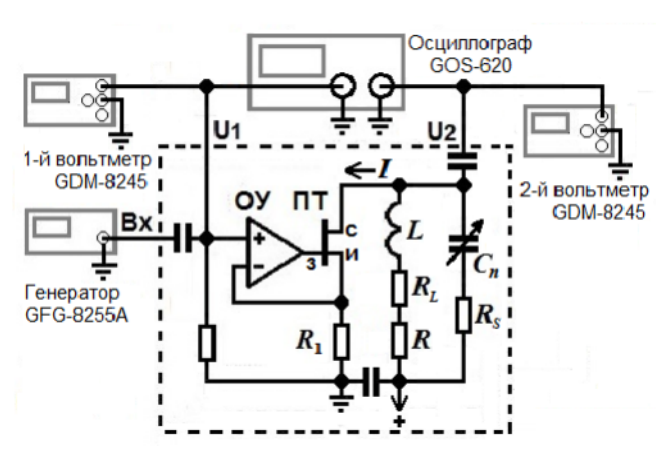
\includegraphics[width=10cm]{fig1.PNG}
    \caption{Схема экспериментального стенда}
    \label{fig:vac}
\end{figure}

Напряжение $ E = E_0cos(\omega t + \phi_0) $ поступает на вход «+» операционного усилителя от генератора через согласующую RC-цепочку. Это же напряжение через разъём «U1» подаётся одновременно на канал 1 осциллографа GOS-620 и вход 1-го цифрового вольтметра GDM-8245. Как видно из схемы, \[ I = \frac{E}{R_1} = I_0cos(\omega t + \phi_0), \:\:\: I_0 = \frac{E_0}{R_1} \]


\section{Ход работы}
\begin{enumerate}
\item Данные установки номер 2: $R = 3,50$ Ом, $R_1 = 1008$ Ом.
    \item Проведём измерения характеристик контура при разных значениях ёмкости конденсатора. Будем фиксировать резонансные частоты $f$ и напряжения $U$ в контуре при разных $C$, так же регистрируя входное напряжение $E$. Результаты измерений занесём в таблицу 1. При расчётах импеданса при резонансе $Z_{res}$, добротности контура $Q$, суммарного сопротивления $R_{\Sigma}$, реактивного сопротивления $\rho$, эквивалентного последовательного сопротивления конденсатора $R_{smax}$ были использованы формулы:\\
    $L = \frac{1}{(2\pi f)^2 C}$, $\rho = \sqrt{\frac{L}{C}}$, $Z_{rez} = \frac{UR_1}{E}$, $Q = \frac{Z_{rez}}{\rho}$, $ R_{sum} = \frac{\rho}{Z_{rez}}$, $ R_{Smax} = 10^{-3}\rho$, $R_{L} = R_{sum} - R_{Smax} - R$\\
    
    \begin{table}[h]
    \centering
    \begin{center}
    \caption{Измерения характеристик контура при разных ёмкостях}
    \end{center}
    \vspace{0.1cm}
    \label{tab:my_label}
    \begin{tabular}{ |p{1.2cm}|p{1.2cm}|p{0.9cm}|p{0.9cm}|p{1.3cm}|p{1.2cm}|p{1.5cm}|p{1.2cm}|p{1.2cm}|p{1.3cm}|p{1.2cm}| }
 \hline
$Cn,$ нФ $\; \; \; \;$& $f,$ кГц & $E,$ В & $U,$ В & $L,$ мкГн & $\rho,$ Ом & $Z_{res},$ Ом & $Q$ & $R_{\Sigma}, $Ом & $R_{Smax}, $Ом & $R_L$, Ом\\
 \hline
25.100 & 32.13 & 0.202 & 1.151 & 978.599 & 197.45 & 5743.6 & 29.08 & 6.78 & 0.197 & 3.09\\
 \hline
33.200 & 27.87 & 0.202 & 0.938 & 981.137 & 172.1 & 4680.71 & 27.19 & 6.33 & 0.172 & 2.65\\
 \hline
47.300 & 23.1 & 0.202 & 0.627 & 996.156 & 145.73 & 3128/79 & 21.47 & 6.79 & 0.146 & 3.14\\
 \hline
57.400 & 21.18 & 0.202 & 0.567 & 977.445 & 130.9 & 2829.38 & 21.6 & 6.06 & 0.131 & 2.43\\
 \hline
67.500 & 19.54 & 0.202 & 0.489 & 989.727 & 120.7 & 2440.15 & 20.21 & 5.97 & 0.121 & 2.35\\
 \hline
82.700 & 17.67 & 0.202 & 0.401 & 977.661 & 108.97 & 2001.03 & 18.36 & 5.93 & 0.109 & 2.32\\
 \hline
101.600 & 16.02 & 0.202 & 0.342 & 965.417 & 97.83 & 2155.72 & 22.03 & 4.44 & 0.098 & 0.84\\
\hline
Ср.знач. & & & & 984,2& & & & & &2.4\\
\hline
Ср.кв.погр. & & & & 3,8& & & & & &0.3\\
\hline
Случайная погр. & & & &5,9 & & & & & &0.3\\
\hline
\end{tabular}
\end{table}
    \item Снимем амплитудно-частотную характеристику контура при ёмкостях $C_2$ и $C_5$. Для этого будем снимать зависимость напряжения в контуре от частоты колебаний. Результаты измерений занесём в табл. (рис.2)\\
    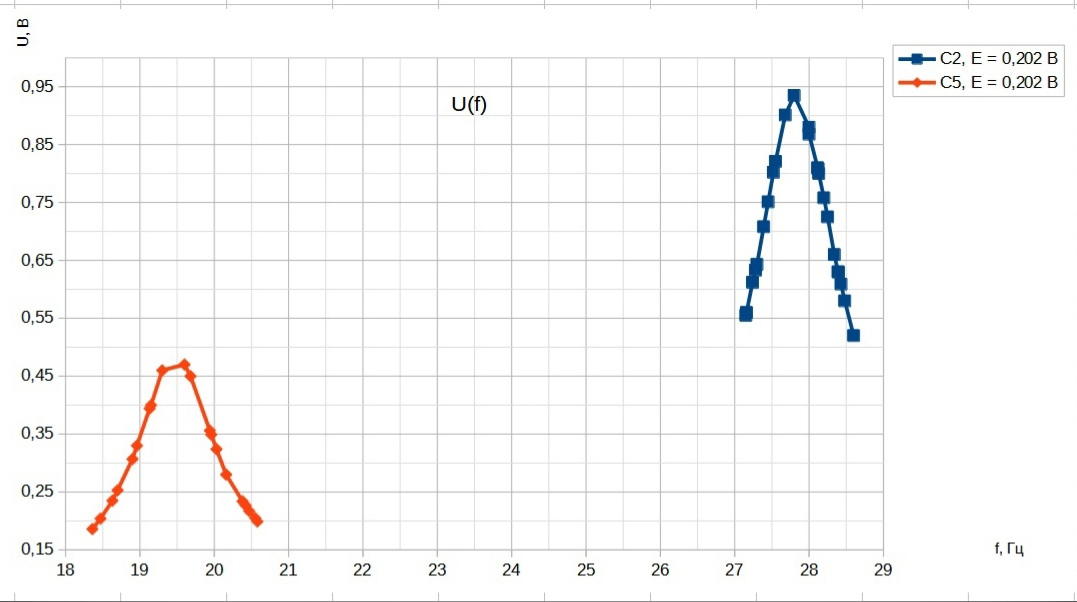
\includegraphics[width=18cm]{g2}\\
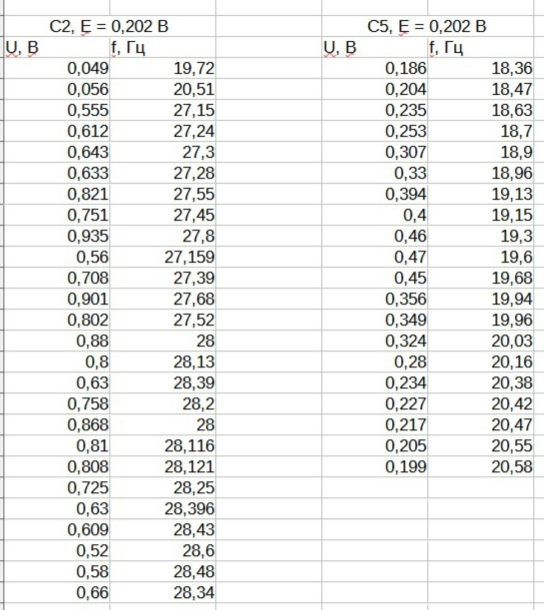
\includegraphics[width=10cm]{g3}\\
    \item Построим графики АЧХ в координатах $U/U_0(f/f_0)$. По этим графикам (ширина резонансной кривой на уровне $\frac{1}{\sqrt{2}}$) определим добротность контуров. $Q = \frac{1}{\delta w}$, где $\delta w$ - ширина резонансной кривой на пересечении с уровнем.\\
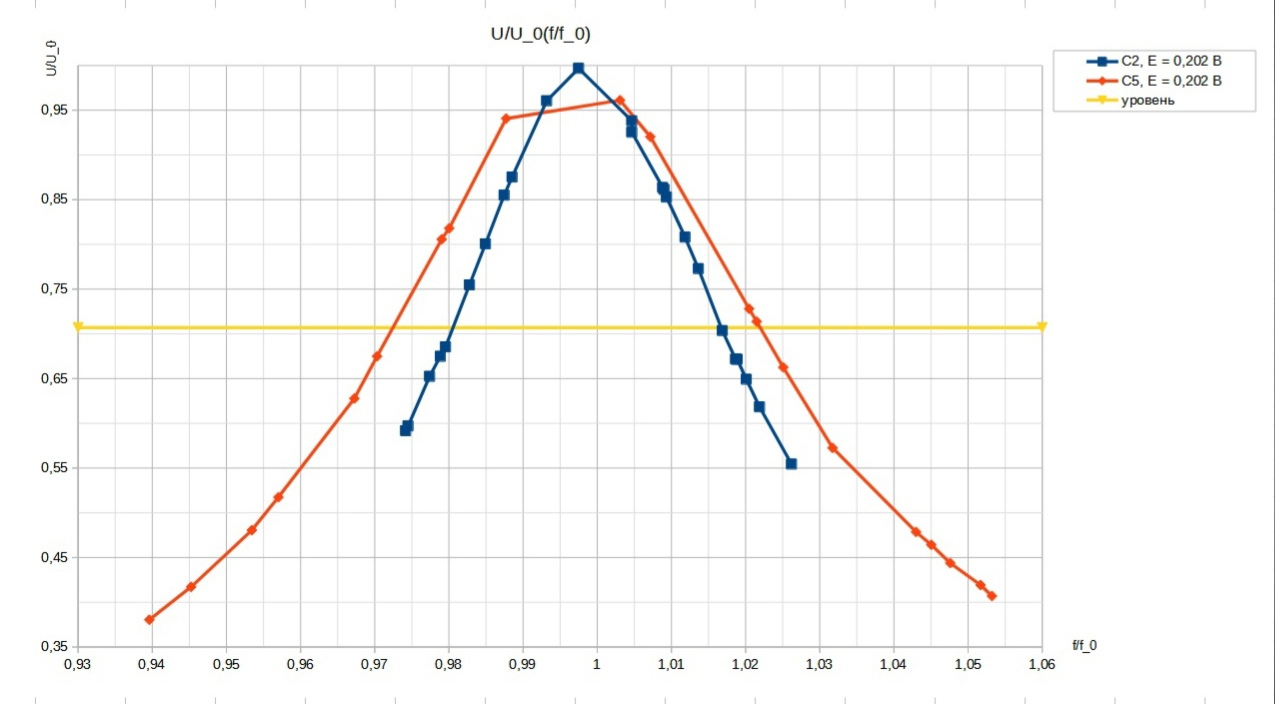
\includegraphics[width=18cm]{g1}\\
\\
Для С2:\\
\fbox{$Q = \frac{1}{0,037} \approx 27,03$}\\
\\
Для С5:\\
\fbox{$Q = \frac{1}{0,0495} \approx 20,2$}\\
\\
Полученные результаты неплохо сходятся теоретическими, вычисленными в первой таблице.\\
    \item Построим ФЧХ для контура с $C_2$ в координатах $x = f/f_0 \;\;\; y = \varphi/\pi$. \\
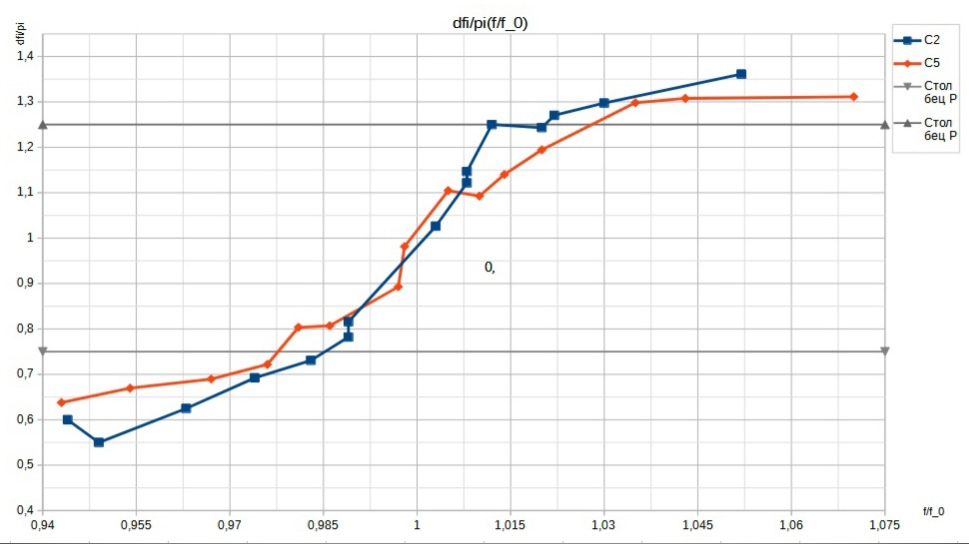
\includegraphics[width=18cm]{g8}\\
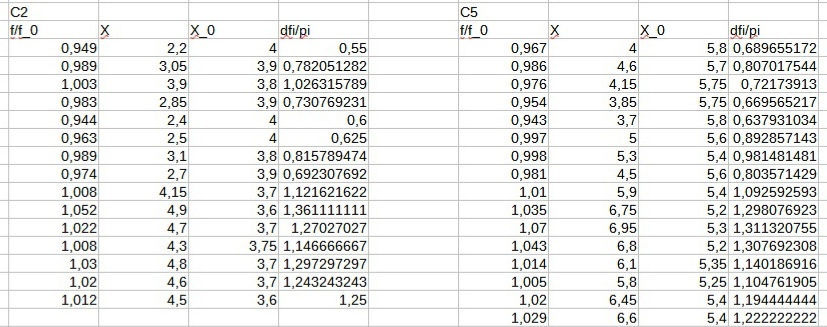
\includegraphics[width=16cm]{g6}\\
    По графику определим добротность контура через расстояние между частотами при разности фаз $\frac{3\pi}{4}$ и $\frac{5\pi}{4}$\\
  \fbox{$Q_2 \approx 33,7$}\\
  \fbox{$Q_5 \approx 20$}\\
  Видим, что результат для $Q_2$ получился несколько завышенным.\\
 \item Построим зависимость $R_L(f)$.\\
 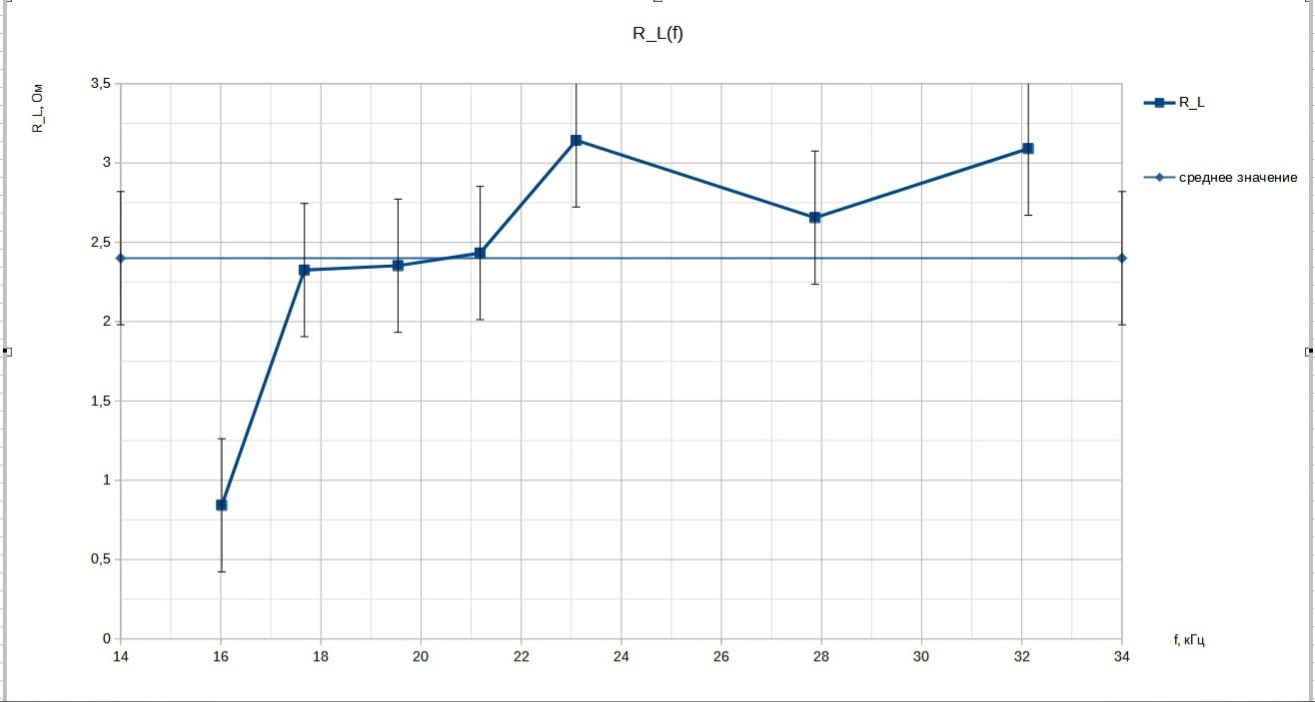
\includegraphics[width = 18cm]{g5}\\
 \\
\item Построим векторную диаграмму для токов и напряжений в контуре с наименьшей добротностью, то есть в контуре 6.\\
Посчитаем ток $ I = \frac{E}{R_1} = \frac{0,202}{1008} \approx 0,1$ мА. Его вектор равен сумме: $ \vec{I} = \vec{I_L} + \vec{I_C} $, причем сам $ \vec{I} $ расположен на оси абсцисс, а его компоненты расположены к нему под углами
\begin{equation}\label{}
\phi_C = \frac{\pi}{2} - \frac{R + R_L}{\rho}, \quad \phi_L = -\frac{\pi}{2} + \delta
\end{equation}
Здесь $ \delta \simeq 10^{-3}$ --- очень малый параметр установки, которым допустимо пренебречь при расчёте, однако можно изобразить для наглядности. Подсчитаем угол $ \phi_C' =   \frac{R + R_l}{\rho} \approx 0,0534 $. 

Аналогичный угол у напряжения $ \vec{U}: \phi_U = - \frac{R + R_l}{\rho} $. Т.е. оно незначительно отклоняется от оси абсцисс на отрицательный угол.
Изобразим это на рисунке. \\
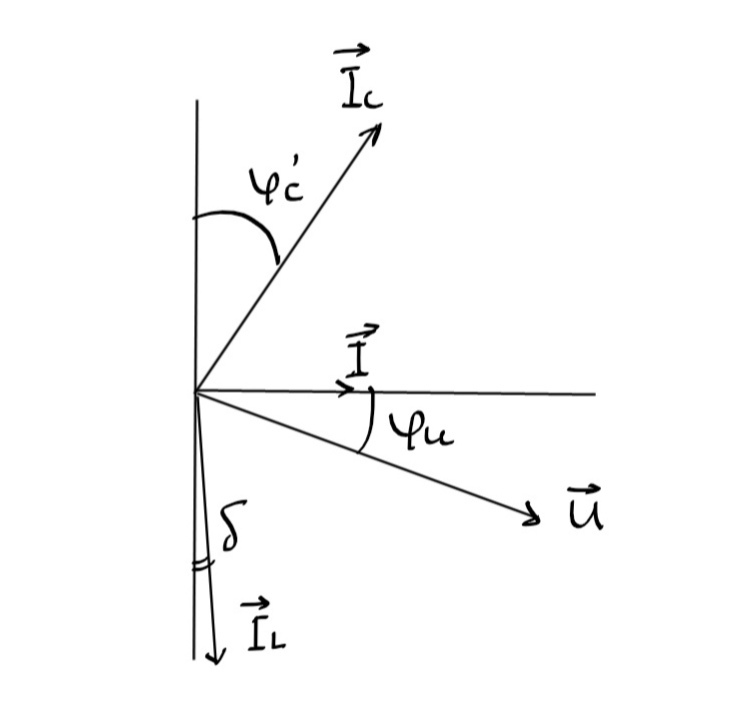
\includegraphics[width=10cm]{g7}\\
\end{enumerate}

\section{Вывод}
В ходе работы мы ознакомились с явлением резонанса токов, изучили метод комплексных амплитуд, изучили амплитудно-частотные и фазово-частотную характеристику колебательного контура, составленного из элементов, используемых в современной радиотехнике.\\
Разными методами была рассчитана добротность колебательного контура при двух различных значениях ёмкости конденсатора в цепи. Полученные результаты с хорошей точностью сходятся между собой:\\
$Q_{2} = 27,19$, $Q_2 = 27,03$, $Q_2 = 33,7$\\
$Q_5 = 20,21$, $Q_5 = 20,2$, $Q_5 = 20$.\\

\end{document}